\documentclass[landscape,12pt]{article}

\usepackage{graphicx}
\usepackage{amssymb}
\newcommand{\slide}[1]{\newpage\noindent{\Huge #1}\\}


\setlength{\pdfpagewidth}{6in}
\setlength{\pdfpageheight}{4.5in}
\setlength{\pdfhorigin}{0.25in}
\setlength{\pdfvorigin}{0.25in}


\setlength{\oddsidemargin}{0in}
\setlength{\topmargin}{-0.5in}
\setlength{\textwidth}{5in}
\setlength{\textheight}{4in}

\begin{document}
\pagestyle{empty}
\sf

\noindent
\mbox{ }
\\[24pt]
{\Huge\bf\sf Known Unknowns in \\[12pt] Discharge Summary Mining}
\\[18pt]
{\Large Bob Carpenter, Breck Baldwin}
\\[6pt]
Alias-i, Inc.
\\[18pt]
{\Large Carlos Cano, Leon Peshkin}
\\[6pt]
Harvard University


\slide{i2b2 Obesity Challenge}

\begin{itemize}
\item
Obesity information and fifteen co-morbidities have been marked at a document
level as:  present (Y), absent (N), questionable (Q), or unmentioned (U)

\item
Two tracks:
  \begin{itemize}
    \item textual judgments, i.e., what the text explicitly states
    \item intuitive judgments, i.e., what the text implies [no U category]
  \end{itemize}

\item
Evaluate systems on their ability to recognize whether a patient is obese
and what co-morbidities they exhibit.

\end{itemize}

\mbox{ }
\\[24pt]
\mbox{ } \hfill {\tt https://www.i2b2.org/NLP/}


\slide{Known Unknowns, Negatives \\[4pt] and Reporting}

\begin{itemize}
\item Questionable (Q) annotations indicated textual or implied
evidence that disease status was unknown (that is, \underline{known unknowns}).
\item Negative (N) annotations in textual judgment means an explicit
recorded negative diagnosis
\item
\begin{tabular}{c|rrrr|r}
Type & Y & N & Q & U & Total \\ \hline
Textual & 3208 & 87 & 39 & 8296 & 11,630 \\
Intuitive & 3267 & 7362 & 26 & n/a & 10,655 \\
\end{tabular}
\item The records aren't being annotated for uncertainty or negative diagnoses
\end{itemize}


\slide{Corpus Adjudication and Agreement}

\begin{itemize}
\item Anonymized discharge summaries from Partners HealthCare for
patients evaluated for obesity or diabetes
\item Annotated by Massachusetts General Hospital Weight Center
\item Two obesity experts independently coded everything
\item One doctor broke ties on textual judgments
\item Intuitive data censored to agreed cases
\item Kappa Scores (P-E)/(1-E)
   \begin{itemize}
   \item Textual Kappas: .71--.92
   \item Intuitive Kappas: .44--.92
   \end{itemize}
\item Training/Test balanced for prevalence of obesity (not co-morbidities)
\end{itemize}


\slide{Evaluation: Macro-Averaged F-Measure}

\begin{itemize}
\item Precision, recall and F-measure for all tasks
\item Ranked by macro-averaged F-measure
  \begin{itemize}
    \item F-measure per morbidity $n$ and type $t \in \{ Y, N, Q, U \}$:  \\[4pt]
          $F_{n,t} = 2 P_{n,t} R_{n,t}/(P_{n,t} + R_{n,t})$
    \item Macro-average per morbidity \\[4pt]
          $F_n = (F_{n,Y} + F_{n,N} + F_{n,Q} + F_{n,U})/4$
    \item Final average for evaluation \\[4pt]
          $F = (F_1 + \cdots F_{16})/16$
  \end{itemize}
\item Low count Q (textual/intuitive) and N (textual) cases heavily weighted
\end{itemize}


\slide{Classification Problem}

\begin{itemize}
\item One classifier per disease
  \begin{itemize}
    \item Textual: Run 1: Y/U,  Runs 2--3: Y/U/N
    \item Intuitive:  Runs 1--3: Y/N
  \end{itemize}
\item Ignored Q cases by misunderstanding task
\end{itemize}

\slide{Multinomial Logistic Regression}
\begin{itemize}
\item Multiple category linear basis classifier (coeffs $\beta \in {\mathbb R}^n$, data $x \in {\mathbb R}^n$)
\[
p(c|x) \propto \mbox{\rm logit}^{-1}(\beta_c x^{\top}) = \frac{1}{1 + \mbox{\rm exp}(-\beta_c x^{\top})}
\]
\item Laplace (double-exponential) priors (aka lasso, $L_1$ regularization)
\[
\log p(\beta) \propto \sum_{1 \leq k \leq n} \frac{|\beta_k|}{\sigma} = \frac{|\beta|_1}{\sigma}
\]
favors zeros but otherwise broader than Gaussian priors
\item Maximum a posteriori (MAP) estimates
\item Optimizes micro-averaged log loss:
\[
\mbox{\rm Err}(\beta) = \log p(\beta) + \sum_i \log p(c_i|x_i)
\]
\item Mismatch with 0/1-loss macro-averaged F-measure
\end{itemize}

\slide{LingPipe's Logistic Regression}

\begin{itemize}
\item Algorithm: Sparse, Regularized Stochastic Gradient Descent (SGD)
\item Online processing; multiple epochs for small data (10K epochs here)
\item Memory: only the coefficients and item being estimated
\item Data vectors may be sparse (here, they're very sparse)
\item General feature extraction interface
\item Built-in implementations of text features (e.g. tokenizers, stemmers, normalizers)
\item Pluggable priors for regularization (Laplace, Cauchy, Gaussian, or user-defined)
\item Fits into LingPipe's classifier evaluation and runtime interfaces
\item Data very close to being linearly separable (near 0 log likelihood)
\end{itemize}



\slide{Run 1: N-gram Features}

\begin{itemize}
\item Character 5-grams
  \begin{itemize}
     \item Input: Anemia and GI bleed.
     \item N-gram Vector: "Anemi":1 "nemia":1, "emia ":1, "mia a":1, "ia an":1, "a and":1, " and ":1, "and G":1, "nd GI":1, "d GI ":1, "GI b":1, "GI bl":1, "I ble":1, " blee":1, "bleed":1, and "leed.":1.
  \end{itemize}
\item Limited cross-word effects
\item Longer n-grams or mixed n-grams didn't help
\item Pruned counts less than 20, resulting in about 20,000 features/task
\item No character normalization (case, punctuation, etc.)
\item Laplace prior variance of 0.1 forces many features to zero
\end{itemize}

\slide{Run 2: Negation and Drug Names}

\begin{itemize}
\item Negative particles distributed over their sentences
as additional features
\begin{verbatim}
IN: no alcohol, tobacco or drug use
ADD: NO_alcohol, NO_tobacco, NO_or, NO_drug, NO_use

IN: No family history of kidney disease or CAD.
ADD: NO_family NO_history NO_of NO_kidney
     NO_disease NO_or NO_CAD
\end{verbatim}
\item LingPipe sentence detection
\item ...
\end{itemize}

\slide{Run 2 (cont.)}
\begin{itemize}
\item Generic drug-treatment feature for drugs used to treat conditions
as additional features (used external knowledge sources to collect synonyms)
\begin{verbatim}
IN: started on clonidine
OUT: Hypertension_DRUG

IN: Clonodine 0.6 mg topical.
ADD: [nothing, it's a misspelling]
\end{verbatim}
\item Pruned to features with counts of 20 or higher
\item Laplace prior further drives parameters to zero
\item Python code to munge input data
\end{itemize}


\slide{Run 3: Feature Selection}

\begin{itemize}
\item Just like Run 2, only selecting limited number of features
\item Information Gain is reduction in entropy (H) of category decisions ($C$) given
the feature $f$ and data $X$:
\[
\mbox{\rm IG}(f) = p(f) \mbox{\rm H}(C|f,X) + (1-p(f)) \mbox{\rm H}(C|\neg f,X)
\]
\[
\mbox{\rm H}(C|f,X) = \sum_{c \in C|f(c)} p(c|X) \log_2 p(c|X)
\]
\item Like an ANOVA (without mixed effects) in log likelihood space
\item Select features with highest IG (greedy and independent)
\item Number of features wasn't sensitive between 5 and 25
\item Reliable general purpose feature selection for text classification
\item Python code to munge input data
\end{itemize}


\slide{Results}

\begin{verbatim}
                                               Accuracy=
Run  Task              P-Mac   R-Mac   F-Mac   P,R,F-Mic

1)   Textual           0.956   0.446   0.451   0.918
2)   Textual           0.567   0.484   0.506   0.923
3)   Textual           0.763   0.457   0.464   0.929

1)   Intuitive         0.928   0.585   0.589   0.902
2)   Intuitive         0.935   0.585   0.592   0.906
3)   Intuitive         0.950   0.600   0.607   0.924
\end{verbatim}

\slide{Conclusions}

\begin{itemize}
\item Most cases very easy (positive obesity very highly correlated
with word ``obese'' in text)
\item Need more data on low-count categories for statistical approach
\item You're only as good as your features
  \begin{itemize}
     \item Need better approach to negation (ideally, parse for scope)
     \item Need better normalization due to case and misspellings
     \item Use structure of document for hierarchical modeling
or feature factorization (e.g. principal diagnosis, secondary diagnoses,
history of present illness, pre-admission meds, past history, family history, social
history, discharge, hospital course, allergies, admission physical exam, studies,
history, etc.)
  \end{itemize}
\item Exploit correlation among output categories
\end{itemize}

\slide{Postscript: Bayesian Diagnosis}

\begin{itemize}
\item $\theta \in [0,1]$: probability of disease
\item $p(\theta)$: prior prevalence in population
\item $X$: observed data (e.g. text, lab reports)
\item $p(X|\theta)$: likelihood (generative)
\item $p(\theta|X) \propto p(X|\theta) p(\theta)$: posterior (by Bayes' law)
\end{itemize}

\slide{Prior Distribution}

\noindent
$p(\theta)$ is an estimate of the population distribution:

\begin{center}
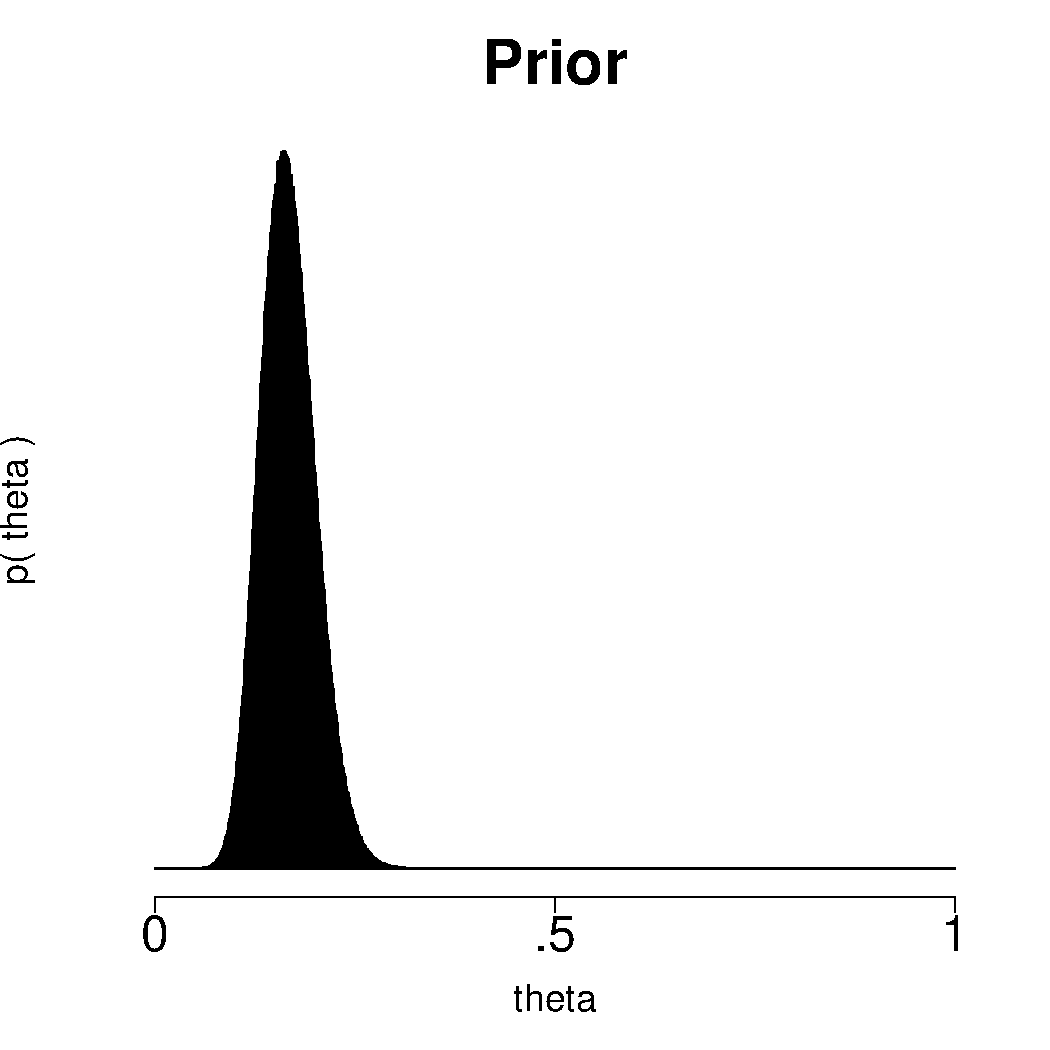
\includegraphics[width=0.5\textwidth]{prior.pdf}
\end{center}

\noindent
$\bullet$ \ Estimate reflects uncertainty in population distribution


\slide{Conclusive Posteriors: Y and N}

\noindent
Posterior is definite in diagnosis

\begin{center}
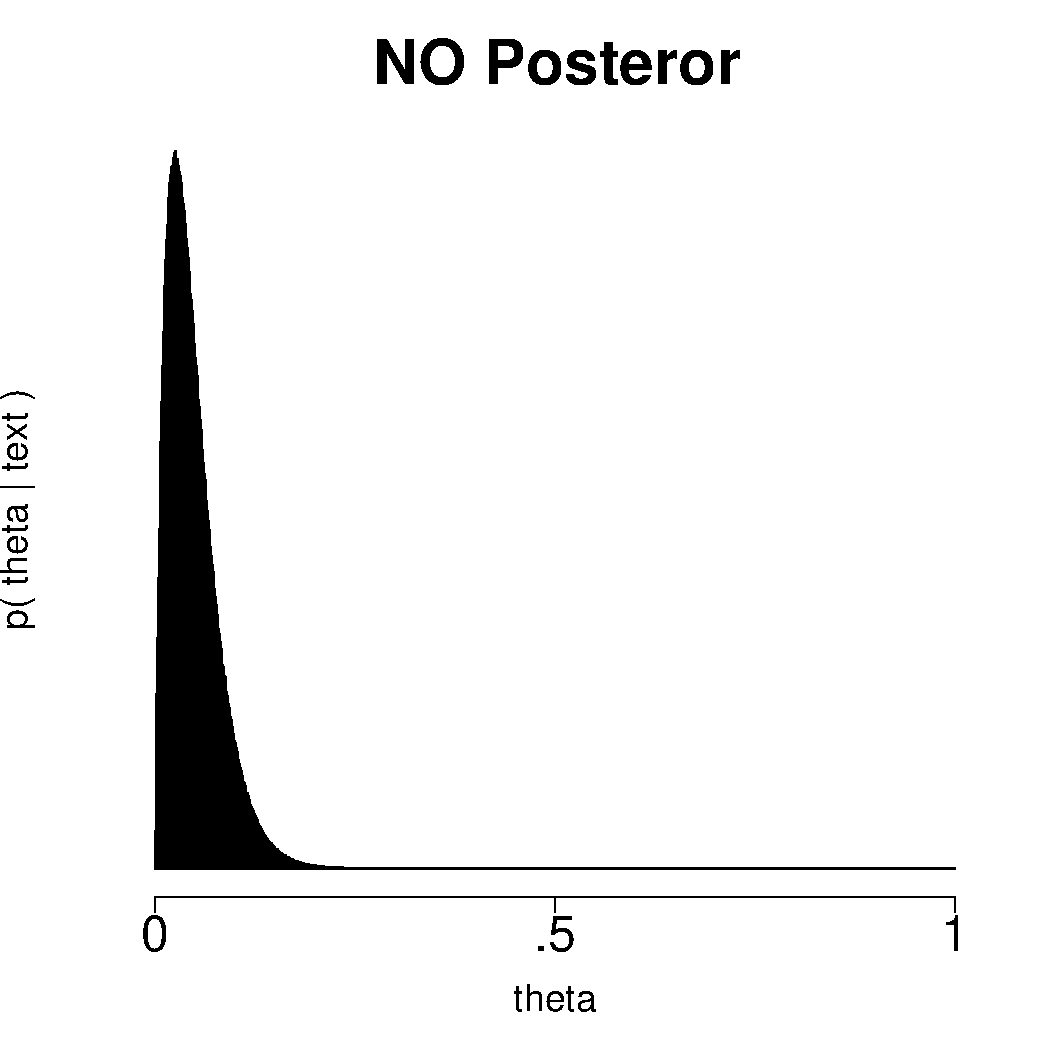
\includegraphics[width=0.4\textwidth]{yes.pdf}
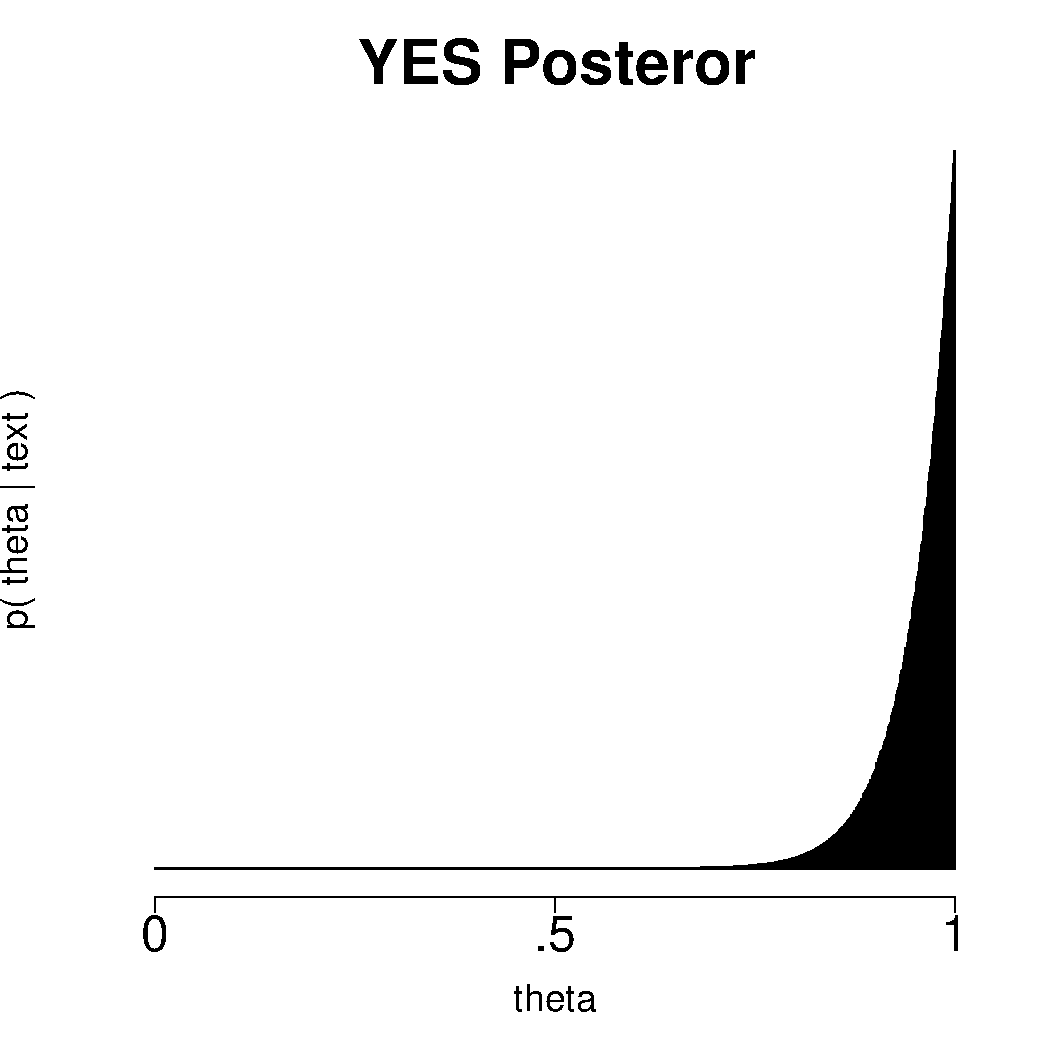
\includegraphics[width=0.4\textwidth]{no.pdf}
\end{center}

\noindent
$\bullet$ \ Estimates reflect posterior uncertainty given data

\noindent
$\bullet$ \ Easy to quantize into discrete categories U and Q


\slide{Inconclusive Posteriors: Q and U}

\noindent Posterior looks like prior for unknowns, more central for borderline/questionable
\begin{center}
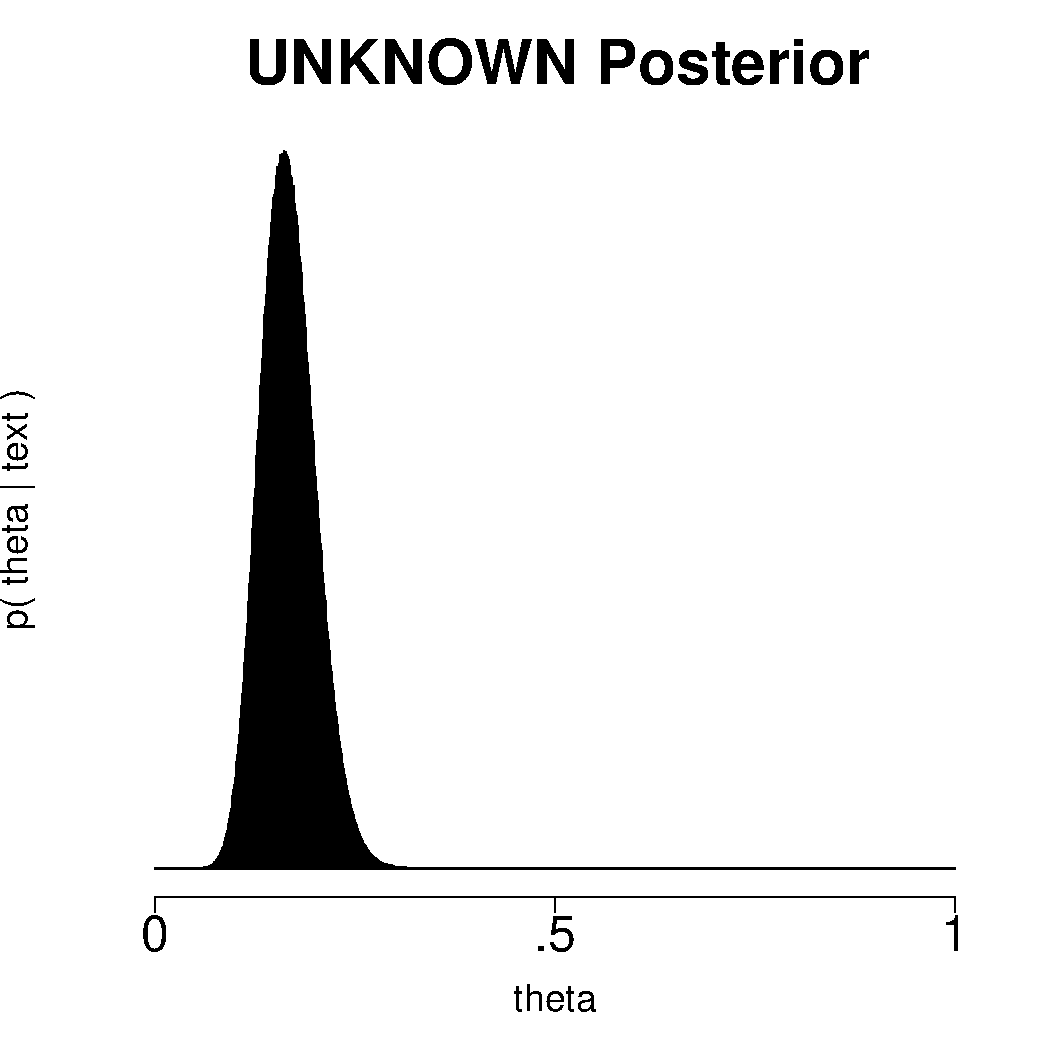
\includegraphics[width=0.4\textwidth]{unknown.pdf}
\includegraphics[width=0.4\textwidth]{questionable.pdf}
\end{center}

\noindent
$\bullet$ \ More difficult to quantize into discrete categories Y and N

\noindent
$\bullet$ \ Still easy to use as a Bayesian component for inference

\slide{Thanks To}

\begin{itemize}
\item Ozlem Uzuner for organizing everything
\item Harvard's i2b2 for hosting
\item NIH for funding
\end{itemize}
\vfill
\noindent
{\it\footnotesize The project described was supported by Grant Number R44 RR020259 from the National Center For Research Resources. The content is solely the responsibility of the authors and does not necessarily represent the official views of the National Center for Research Resources or the National  Institutes of Health.}

\end{document}